\section{Краткие теоретические сведения}

Смысл атаки <<Человек посередине>> (от англ. Man-in-the-middle, MITM) заключается в том, что злоумышленник проксирует часть сетевого трафика жертвы через себя. В то время пока жертва считает, что работает напрямую, к примеру, с веб-сайтом своего банка, трафик проходит через промежуточный узел злоумышленника, который таким образом получает  отправляемые пользователем данные.

Атака обычно начинается с прослушивания канала связи и заканчивается тем, что злоумышленник пытается подменить перехваченное сообщение, извлечь из него полезную информацию и перенаправить его на какой-нибудь внешний ресурс.

\begin{figure}[H]
	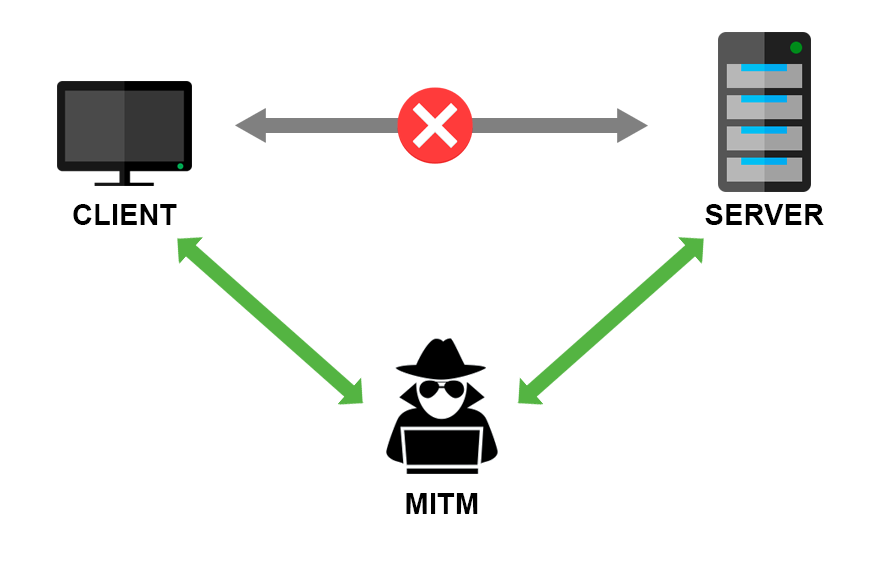
\includegraphics[width=.9\textwidth]{img/mitm.png}
	\caption{Атака типа <<Человек посередине>>}
\end{figure}

Одним из примеров атак типа <<человек посередине>> является активное прослушивание, при котором злоумышленник устанавливает независимые связи с жертвами и передаёт сообщения между ними. Тем самым он заставляет жертв поверить, что они разговаривают непосредственно друг с другом через частную связь, фактически же весь разговор управляется злоумышленником. Злоумышленник должен уметь перехватывать все передаваемые между двумя жертвами сообщения, а также вводить новые. В большинстве случаев это довольно просто, например, злоумышленник может вести себя как <<человек посередине>> в пределах диапазона приёма беспроводной точки доступа.

Данная атака направлена на обход взаимной аутентификации или отсутствие таковой и может увенчаться успехом только тогда, когда злоумышленник имеет возможность выдать себя за каждую конечную точку либо оставаться незамеченным в качестве промежуточного узла. Большинство криптографических протоколов включает в себя некоторую форму аутентификации конечной точки специально для предотвращения MITM-атак. 